\graphicspath{ {./images/3_Spectra_curation} }
\newpage

\section{Spectra curation}
\subsection{Choosing analyte quality criteria}
The analyte quality criteria are used to judge whether the signal of an analyte is of sufficient quality in a given sample to be reliably quantified.
It is important to note that different charge states for the same glycopeptide are treated as distinct analytes. 
This information is used for spectra curation and for the subsequent analyte curation step. 
Depending on the type of data uploaded, there are three distinct quality criteria for which boundaries can be configured.
An analyte is deemed to be of sufficient quality when it meets all three criteria. 
Only in very specific cases, one or two of the listed quality criteria may be used, by clicking the gears icon and deselecting the criteria that you wish to ignore.

\subsubsection{LaCyTools or SweetSuite data}
\begin{wrapfigure}{R}{0.37\textwidth}
	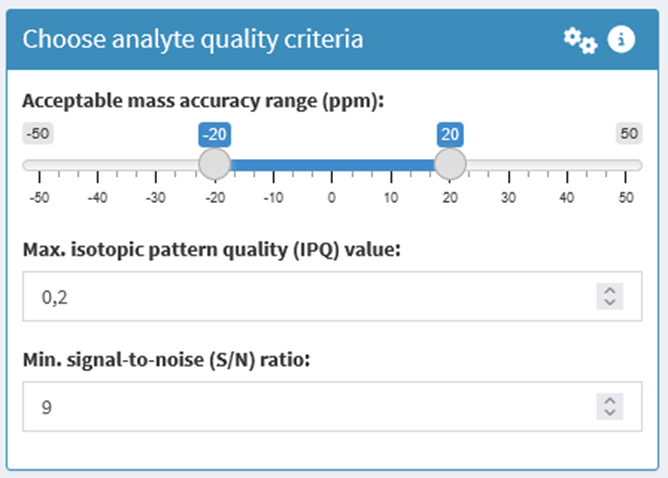
\includegraphics[scale = 0.35]{qc1.png}
 \end{wrapfigure}
Three quality criteria can be set for LaCyTools and SweetSuite data:

\begin{itemize}[topsep=0pt, itemsep=0pt]
	\item \textsf{Acceptable mass accuracy range (ppm)} \\
	Sets the acceptable mass accuracy (mass error) in parts-per-million (ppm).
	The maximum range is $-50$ to $+50$ ppm, with the default being $-20$ to $+20$ ppm.
	\item \textsf{Maximum isotopic pattern quality (IPQ) value} \\
	Sets the maximum acceptable IPQ value for an analyte.
	The lower the IPQ value of an analyte, the better the observed isotopic pattern of that analyte matches the theoretical isotopic pattern.
	The default value is $0.2$.
	\item \textsf{Maximum signal-to-noise ($S/N$) ratio} \\
	The minimum $S/N$ ratio that an analyte should have to be considered of sufficient quality.
	The default value is $9$.
\end{itemize}


\subsubsection{Skyline data}
\begin{wrapfigure}{R}{0.37\textwidth}
	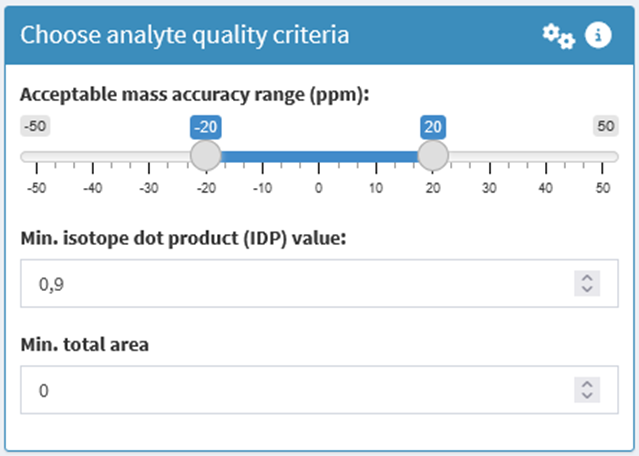
\includegraphics[scale = 0.35]{qc2.png}
\end{wrapfigure}
Three quality criteria can be set for Skyline data:

\begin{itemize}[topsep=0pt, itemsep=0pt]
	\item \textsf{Acceptable mass accuracy range (ppm)} \\
	Sets the acceptable mass accuracy (mass error) in parts-per-million (ppm).
	The maximum range is $-50$ to $+50$ ppm, with the default being $-20$ to $+20$ ppm.
	\item \textsf{Minimum isotope dot product (IDP) value} \\
	The minimum IDP value that an analyte should have.
	The higher the IDP value, the better the observed isotopic pattern of an analyte matches its theoretical isotopic pattern.
	The IDP can have a maximum value of 1, indicating a perfect match.
	The default minimum value is set to $0.9$.
	\item \textsf{Minimum total area} \\
	As Skyline does not output $S/N$ values, the total area can be used as an alternative.
	By default, this values is set to 0 (i.e. it is ignored).
\end{itemize}


\newpage
\subsection{Spectra curation cut-offs}
For each sample and glycosylation site in your data, the intensities of all analytes fulfilling the set QC parameters are summed, and the percentage of passing analytes out of all targeted analytes is calculated. 
Each spectrum will be curated based on these values. 
The two available methods for curating the spectra are described below.
Alternatively, you have the option to skip spectra curation, in which case all spectra will be utilized in subsequent processing steps.

\subsubsection{Curate spectra based on negative controls}
First, choose which sample types should be used as negative controls.
Then set a percentile of negative control measurements for calculating cut-off values.
The default percentile is set to 95.
Cut-off values will be computed for both the ``sum intensity'' and ``percentage of passing analytes'' values.
These cut-offs are calculated separately for each glycosylation site.

\begin{optionalbox}
	By default, uncalibrated spectra are treated as having missing values and will be excluded from the calculations.
	It is possible to include them with a value of zero by unchecking the \menu{Treat uncalibrated spectra as missing values, not zeros} option.
\end{optionalbox}

During curation, spectra whose percentage of passing analytes and sum intensity exceed or equal the corresponding cut-off values will pass curation.
These passing spectra will be used for further data processing.
In the \textsf{Perform spectra curation} box, all spectra are displayed per glycosylation site in an interactive plot, color-coded by sample type.
The cut-off values are indicated by dashed bars, and the exact cut-off values are displayed below the plot.

When satisfied with the cut-off values, click on \menu{Perform spectra curation}

\begin{optionalbox}
	It is possible to set manual cut-offs for a glycosylation site by toggling the \menu{\textsf{Set cut-offs manually}} option in the corresponding tab.
\end{optionalbox}

\begin{center}
	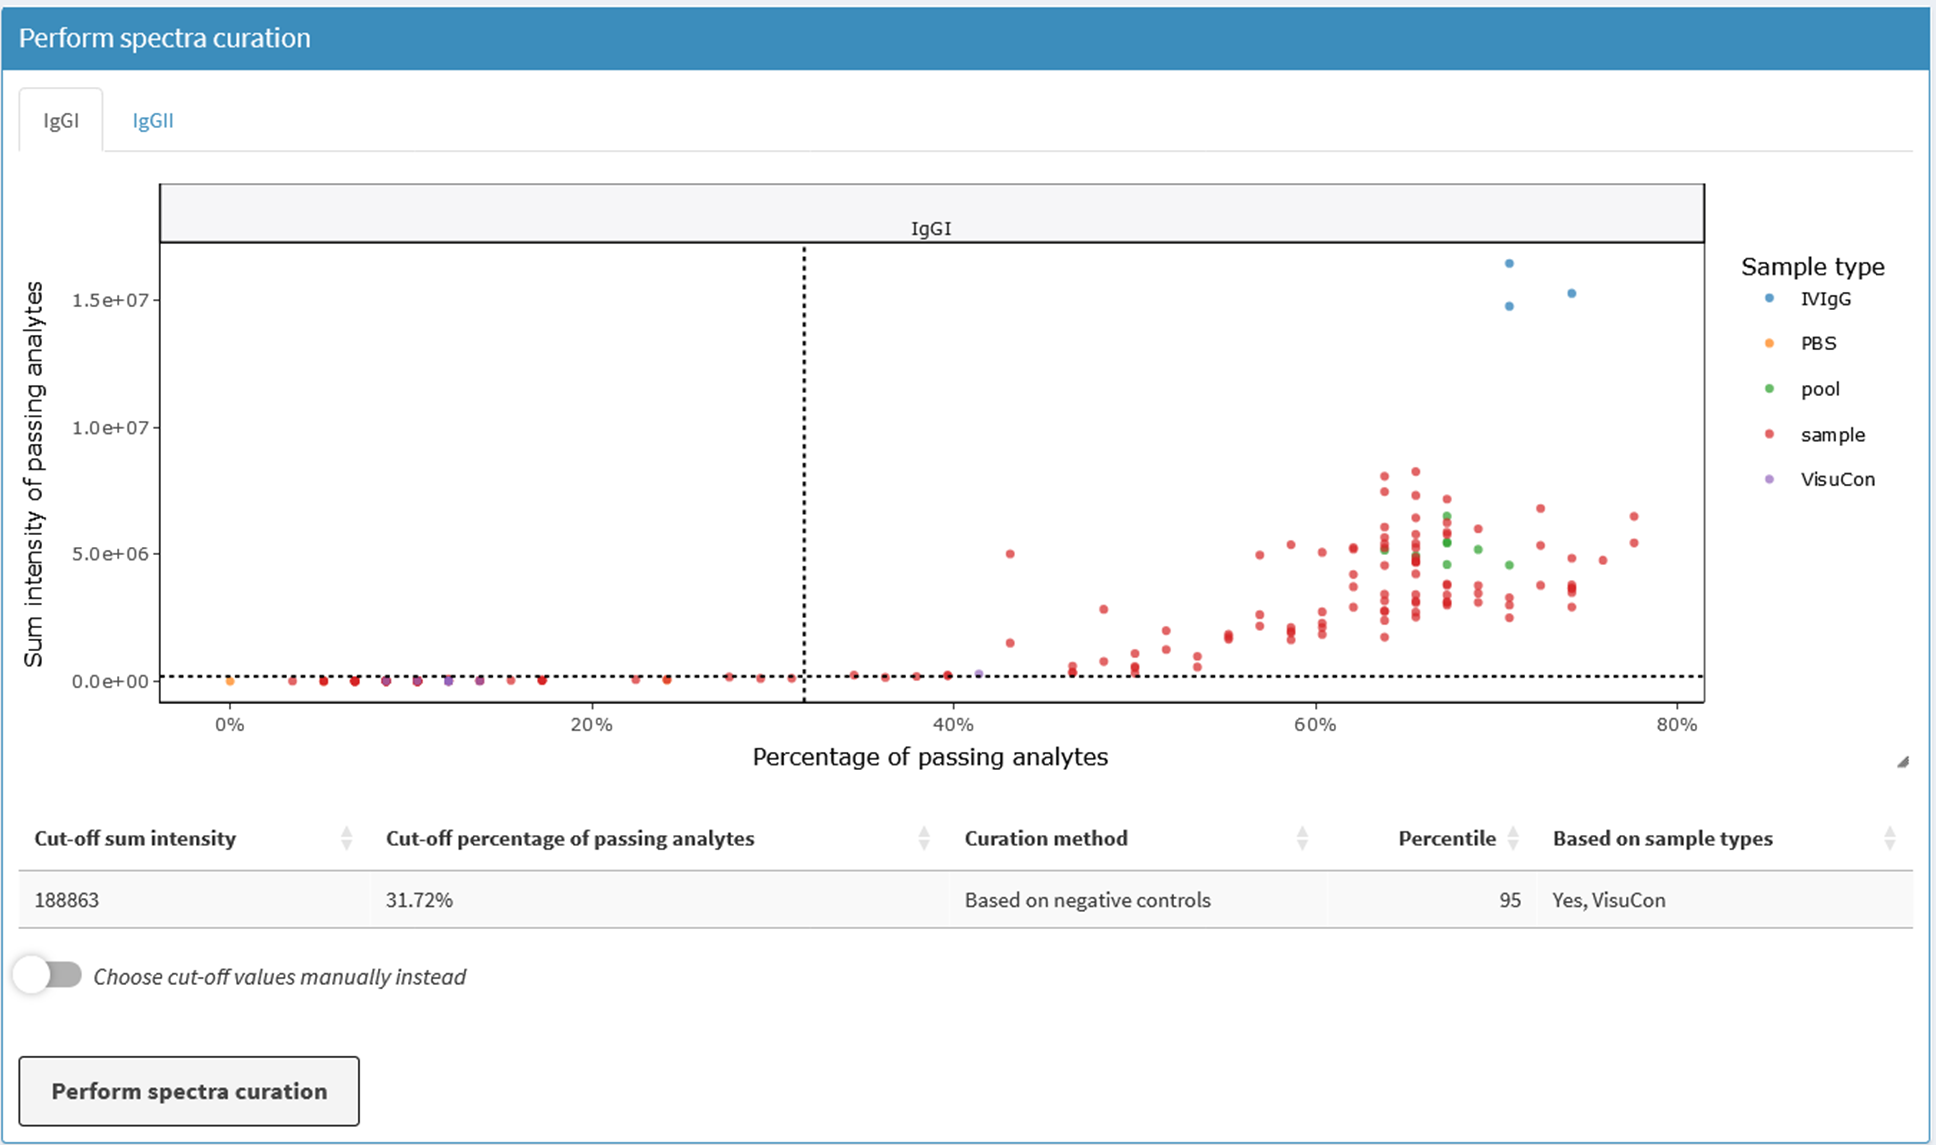
\includegraphics[scale=0.29]{perform_curation.png}
\end{center}



\newpage
\subsubsection{Curate spectra based on percentiles}
In this scenario, cut-off values are determined at a set percentile based on all measurements associated with a glycosylation site, with the option to exclude a selection of sample types from the calculation.
Using this method, a fixed proportion of all data (that of the lowest quality) will be excluded from further processing.

\begin{enumerate}[topsep=0pt, itemsep=0pt]
	\item Choose the percentile at which to set the cut-off values. 
	The default value is set to 5.
	\item Optionally, exclude certain sample types from the calculations.
	It is recommended to exclude all types of control samples.
	Excluded samples will still be curated based on the calculated cut-off values.
	\item Review the cut-off values in the \textsf{Perform spectra curation} box.
	\item When satisfied with the cut-offs, click on \menu{Perform spectra curation}.
\end{enumerate}


\subsection{Spectra curation results}
After performing spectra curation, an interactive plot displaying the results is generated. 
The plot shows the percentage of passing and failing spectra for each sample type per glycosylation site.
The reasons for failing curation are indicated by different colors.
For LaCyTools and SweetSuite output, the percentage of uncalibrated spectra is also displayed (this calibration step can be seen as a first-pass spectra curation).

\begin{center}
	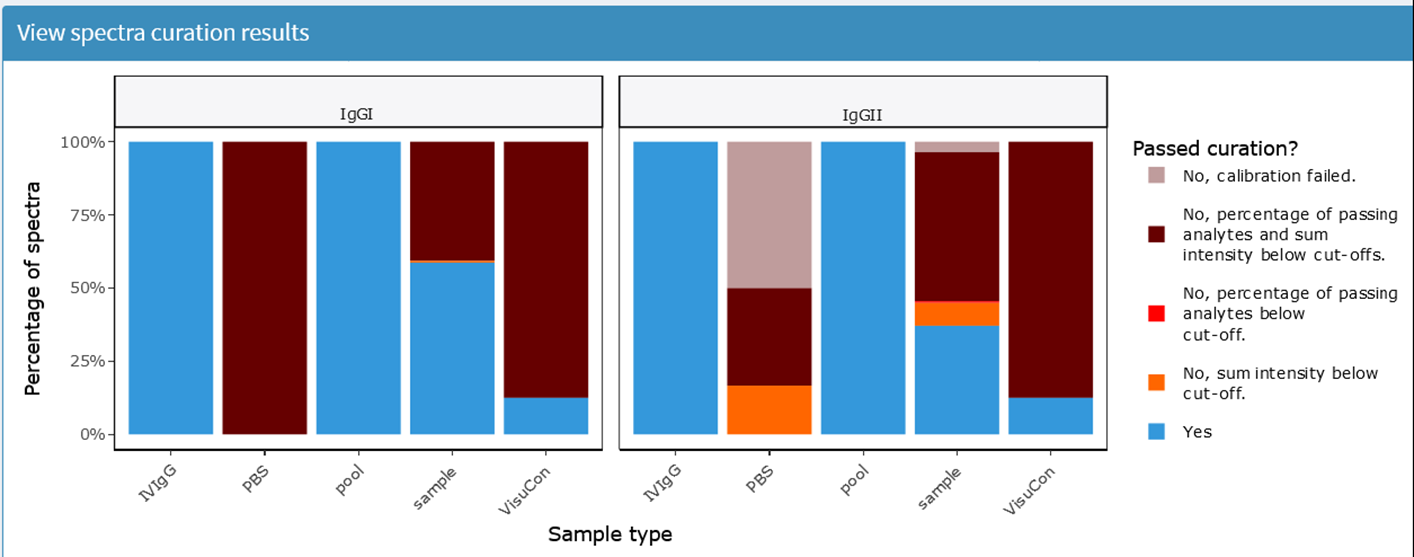
\includegraphics[scale=0.42]{curation_results.png}
\end{center}

Below the plots, three tables are shown displaying the following information:

\begin{itemize}[topsep=0pt, itemsep=0pt]
	\item Details of passing spectra per analyte.
	\item Overview of failed spectra.
	\item Details of failed spectra per analyte.
\end{itemize}

There is an option to download each of these tables as a \texttt{.xlsx} file, at the bottom of the page in the \textsf{Export results} box.



